\documentclass[a4paper,12pt]{article}
\usepackage[top = 2.5cm, bottom = 2.5cm, left = 2.5cm, right = 2.5cm]{geometry}
\usepackage[T1]{fontenc}
\usepackage[utf8]{inputenc}
\usepackage{multirow} 
\usepackage{booktabs} 
\usepackage{graphicx}
\usepackage[spanish]{babel}
\usepackage{setspace}
\setlength{\parindent}{0in}
\usepackage{float}
\usepackage{fancyhdr}
\usepackage{amsmath}
\usepackage{amssymb}
\usepackage{amsthm}
\usepackage[numbers]{natbib}
\newcommand\Mycite[1]{%
	\citeauthor{#1}~[\citeyear{#1}]}
\usepackage{graphicx}
\usepackage{subcaption}
\usepackage{booktabs}
\usepackage{etoolbox}
\usepackage{minibox}
\usepackage{hyperref}
\usepackage{xcolor}
\usepackage[skins]{tcolorbox}
%---------------------------

\newtcolorbox{cajita}[1][]{
	 #1
}

\newenvironment{sol}
{\renewcommand\qedsymbol{$\square$}\begin{proof}[\textbf{Solución.}]}
	{\end{proof}}

\newenvironment{dem}
{\renewcommand\qedsymbol{$\blacksquare$}\begin{proof}[\textbf{Demostración.}]}
	{\end{proof}}

\newtheorem{problema}{Problema}
\newtheorem{definicion}{Definición}
\newtheorem{ejemplo}{Ejemplo}
\newtheorem{teorema}{Teorema}
\newtheorem{corolario}{Corolario}[teorema]
\newtheorem{lema}[teorema]{Lema}
\newtheorem{prop}{Proposición}
\newtheorem*{nota}{\textbf{NOTA}}
\renewcommand\qedsymbol{$\blacksquare$}
\usepackage{svg}
\usepackage{pgfplots}
\pgfplotsset{compat=1.11}

\usepackage{tikz}
\usetikzlibrary{calc}

\usetikzlibrary{patterns}
\usepackage[framemethod=default]{mdframed}
\global\mdfdefinestyle{exampledefault}{%
linecolor=lightgray,linewidth=1pt,%
leftmargin=1cm,rightmargin=1cm,
}




\newenvironment{noter}[1]{%
\mdfsetup{%
frametitle={\tikz\node[fill=white,rectangle,inner sep=0pt,outer sep=0pt]{#1};},
frametitleaboveskip=-0.5\ht\strutbox,
frametitlealignment=\raggedright
}%
\begin{mdframed}[style=exampledefault]
}{\end{mdframed}}
\newcommand{\linea}{\noindent\rule{\textwidth}{3pt}}
\newcommand{\linita}{\noindent\rule{\textwidth}{1pt}}

\AtBeginEnvironment{align}{\setcounter{equation}{0}}
\pagestyle{fancy}

\fancyhf{}









%----------------------------------------------------------
\lhead{\footnotesize Geometría diferencial}
\rhead{\footnotesize  Rudik Roberto Rompich}
\cfoot{\footnotesize \thepage}


%--------------------------

\begin{document}
 \thispagestyle{empty} 
    \begin{tabular}{p{15.5cm}}
    \begin{tabbing}
    \textbf{Universidad del Valle de Guatemala} \\
    Departamento de Matemática\\
    Licenciatura en Matemática Aplicada\\\\
   \textbf{Estudiante:} Rudik Roberto Rompich\\
   \textbf{Correo:}  \href{mailto:rom19857@uvg.edu.gt}{rom19857@uvg.edu.gt}\\
   \textbf{Carné:} 19857
    \end{tabbing}
    \begin{center}
        Geometría diferencial - Catedrático: Alan Reyes\\
        \today
    \end{center}\\
    \hline
    \\
    \end{tabular} 
    \vspace*{0.3cm} 
    \begin{center} 
    {\Large \bf  Tarea
} 
        \vspace{2mm}
    \end{center}
    \vspace{0.4cm}
%--------------------------


\begin{problema}
    Sea
    \begin{enumerate}
        \item Sea $\alpha(t)$ una curva parametrizada en $\mathbb{R}^{n}$, que no pasa por el origen $O$. Si $\alpha\left(t_{0}\right)$ es un punto del trazo de $\alpha$ que está más próximo a $O$, y $\alpha^{\prime}\left(t_{0}\right) \neq 0$ entonces $\alpha\left(t_{0}\right)$ es ortogonal a $\alpha^{\prime}\left(t_{0}\right)$
            \begin{sol}
                Sea $\alpha: I\to \mathbb{R}^n$ tal que $\alpha(t)=(x_1(t),x_2(t),\cdots, x_n(t))$. A probar: $\langle\alpha(t), \alpha'(t)\rangle=0$. Considerando la definición de norma, la cual es la distancia del origen $O$ a los puntos $(x_1(t),x_2(t),\cdots, x_n(t))$, se tiene: 
                $$\|\langle \alpha(t),\alpha(t)\rangle\|=\sqrt{\langle\alpha(t),\alpha(t)\rangle}=\sqrt{x_1^2(t)+x_2(t)^2+\cdots x_n^2(t)}$$
                Sin embargo, deseamos encontrar una relación del producto interno, entonces, considérese: $f:I\to \mathbb{R}^n$ tal que: 
                $$f(t)=\|\langle \alpha(t),\alpha(t)\rangle\|^2=\langle\alpha(t),\alpha(t)\rangle=x_1^2(t)+x_2(t)^2+\cdots x_n^2(t)$$

                Además, de la hipótesis, también tenemos que $\alpha(t_0)$ es un punto del trazo de $\alpha$ que está más próximo al origen $O$, es decir que es un mínimo local en $t_0\implies f'(t_0)=0$. Con eso, la considérese la derivada de $f(t)$,
                \begin{align*}
                    f'(t)&=\frac{d\langle \alpha(t),\alpha(t)\rangle}{dt}\\
                         &= \langle \alpha'(t),\alpha(t)\rangle+\langle \alpha(t),\alpha'(t)\rangle\\
                         &= 2 \langle \alpha'(t),\alpha(t)\rangle
                \end{align*}
                Consideramos el punto $t_0$ tal que: 
                \begin{align*}
                    f'(t_0)&= 2 \langle \alpha'(t_0),\alpha(t_0)\rangle=0
                \end{align*}
                Por lo tanto, $$\langle\alpha(t), \alpha'(t)\rangle=0.$$
            \end{sol}
        \item Sea $\alpha: I \rightarrow \mathbb{R}^{3}$ una curva parametrizada, con $\alpha^{\prime}(t) \neq 0, \forall t \in I$. Mostrar que $\|\alpha(t)\|$ es una constante $>0$ si, y sólo si, $\alpha(t)$ es ortogonal a $\alpha^{\prime}(t)$, para todo $t \in I$.
        \begin{sol}
            Procedemos por doble implicación:
            \begin{itemize}
                \item $(\implies)$ A probar: $\langle\alpha(t),\alpha'(t)\rangle =0 $. Sea por hipótesis,
                \begin{align*}
                    \|\alpha(t)\|&= C\\
                    \|\alpha(t)\|^2&= C^2\\
                    \frac{d}{dt}\|\alpha(t)\|^2&= \frac{d}{dt}C^2\\
                    \frac{d}{dt}\langle\alpha(t),\alpha(t)\rangle &= 0\\
                    2 \langle \alpha'(t),\alpha(t)\rangle &=0\\
                    \langle \alpha'(t),\alpha(t)\rangle &=0
                \end{align*}
                
                \item $(\impliedby)$ A probar: $\|\alpha(t)\|=C>0.$ Por el inciso anterior, nótese que esta implicación también se cumple. 
            \end{itemize}
        \end{sol}
    \end{enumerate}
    
\end{problema}

\begin{problema}
    Considere la parametrización de la cicloide de radio $r$ vista en aula.
    \begin{figure}[H]
        \centering
        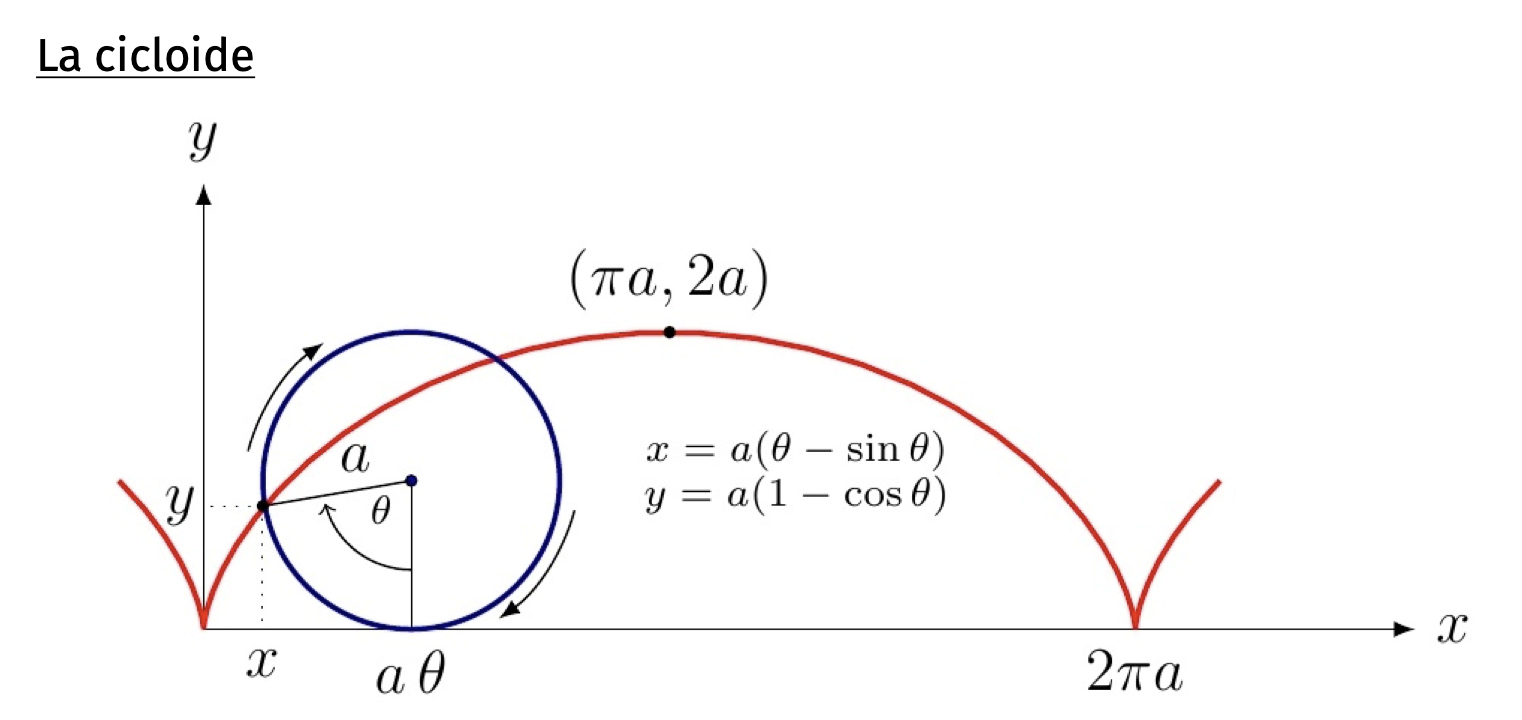
\includegraphics[scale=0.5]{Problemas/cicloide.png}
        \caption{Parametrización vista en clase}
    \end{figure}
    \begin{enumerate}
        \item Calcular la longitud de arco de la cicloide en el primero de sus arcos, esto es correspondiente a una rotación completa del círculo.
        \begin{sol}
            Sea 
            $$\alpha(\theta) = \left(a\left(\theta -\sin \theta\right),a(1-\cos\theta)\right)$$
            En donde, 
            $$\alpha'(\theta)=\left(a\left(1 -\cos \theta\right),
            a\sin \theta\right) $$
            Considérese: 
            \begin{align*}
                s(t) &= \int_{t_0}^{t}|\alpha'(\theta)|d\theta\\
                &= \int_0^{2\pi}\sqrt{\left[a(1-\cos\theta)\right]^2 + \left[a\sin\theta\right]^2}d\theta\\
                &=  \int_0^{2\pi}\sqrt{a^2\left[(1-\cos \theta)^2+\sin^2\theta\right]}d\theta\\
                &= a\int_0^{2\pi}\sqrt{1-2\cos\theta +\cos^2\theta +\sin^2\theta }d\theta\\
                &= a\int_0^{2\pi}\sqrt{2(1-\cos\theta)}d\theta\\
                &= a\sqrt{2}\int_0^{2\pi}\sqrt{1-\cos\theta}d\theta\\
                &= a\sqrt{2}\int_0^{2\pi}\sqrt{2\sin^2\frac{\theta}{2} }d\theta\\
                &= 2a \int_0^{2\pi}\sin \frac{\theta}{2}d\theta\\
                &= 2a(4)= 8a 
            \end{align*}
        \end{sol}

        \item Calcular el área bajo la curva (entre la curva y el eje $x$) para este arco de cicloide.
        \begin{sol}
            Considérese, la ecuación para calcular el área de una curva paramétrica: 
            \begin{align*}
                A &= \int_0^{2\pi a} y dx
                \intertext{Donde $dx = a(1-\cos \theta)d\theta $}
                A &= \int_0^{2\pi}\left(a(1-\cos\theta)\right)\left(a(1-\cos \theta)d\theta \right)\\
                &= a^2\int_0^{2\pi}\left(1-\cos\theta\right)^2d\theta = a^2\int_0^{2\pi}\left(1-2\cos\theta +\cos^2\theta \right)d\theta \\
                &= a^2\int_0^{2\pi}\left(1-2\cos\theta +\frac{1}{2}\cos 2\theta +\frac{1}{2}\right)d\theta \\
                &= a^2\int_0^{2\pi}\left(-2\cos\theta +\frac{1}{2}\cos 2\theta +\frac{3}{2}\right)d\theta \\
                &= a^2 \left[-2\sin\theta +\frac{1}{4}\left(\sin 2\theta \right)+\frac{3}{2}\theta \right]_0^{2\pi }\\
                &= a^2 \left[-2(\sin 2\pi -\sin 0)+\frac{1}{4}(\sin 4\pi -\sin 0)+\frac{3}{2}(2\pi - 0)\right]\\
                &= a^2(3\pi ) = 3\pi a^2
            \end{align*}
        \end{sol}
    \end{enumerate}


\end{problema}

\begin{problema}
 Sea $\alpha:(0, \pi) \rightarrow \mathbb{R}^{2}$ la curva dada por

$$
\left(\sin t, \cos t+\log \tan \frac{t}{2}\right),
$$

donde $t$ es el ángulo que el eje $y$ con el vector $\alpha^{\prime}(t)$. Esta curva se llama la tractriz (Figura en pág. 8 de Do Carmo). Mostrar que

\begin{itemize}
    \item $\alpha$ es una curva parametrizada diferenciable, regular excepto en $t=\frac{\pi}{2}$.
    \begin{sol}
        Proponemos la derivada de $\alpha(t)$,
        \begin{align*}
            \alpha'(t)&=\left(\cos t, -\sin t +\frac{1}{\tan \frac{t}{2}}\cdot \sec^2 \frac{t}{2}\cdot \frac{1}{2}\right)\\
            &= \left(\cos t, -\sin t +\frac{1}{\frac{\sin \frac{t}{2} }{\cos \frac{t}{2}}}\cdot \left(\frac{1}{\cos \frac{t}{2}}\right)^2 \cdot \frac{1}{2}\right)\\
            &= \left(\cos t, -\sin t +\frac{1}{\sin \frac{t}{2} }\cdot \frac{1}{\cos \frac{t}{2}} \cdot \frac{1}{2}\right)\\
            &= \left(\cos t, -\sin t +\frac{1}{\sin t}\right)\\
        \end{align*}

        Ahora, mostraremos que es diferenciable regular en $t\in (0,\pi)$ excepto en $t=\pi/2$. Es decir, que solamente en  $\alpha'(\pi/2)=0$.
        \begin{align*}
            \alpha'(\pi/2)&= \left(\cos \frac{\pi}{2}, -\sin \frac{\pi}{2} +\frac{1}{\sin \frac{\pi}{2}}\right)\\
            &= \left(0, -1 +1\right)\\
            &= \left(0, 0\right)
        \end{align*}

        Entonces,
        \begin{align*}
            \cos t &= 0\\
            t &= \arccos 0\\
            t &= \frac{\pi}{2}
        \end{align*}
        y 
        \begin{align*}
            -\sin t +\frac{1}{\sin t}&=0\\
            -\sin t &=-\frac{1}{\sin t}\\
            \sin^2 t &= 0\\
            \sin t & = 0\\
            t &= \arcsin 0\\
            t &= \frac{\pi}{2}
        \end{align*}

    \end{sol}
    \item La longitud del segmento de la tangente a la tractriz, entre el punto de tangencia y el eje $O y$ es constante e igual a 1.
    \begin{sol}
        Debemos mostrar que los segmentos rojos son 1. 
        \begin{figure}[H]
            \centering
            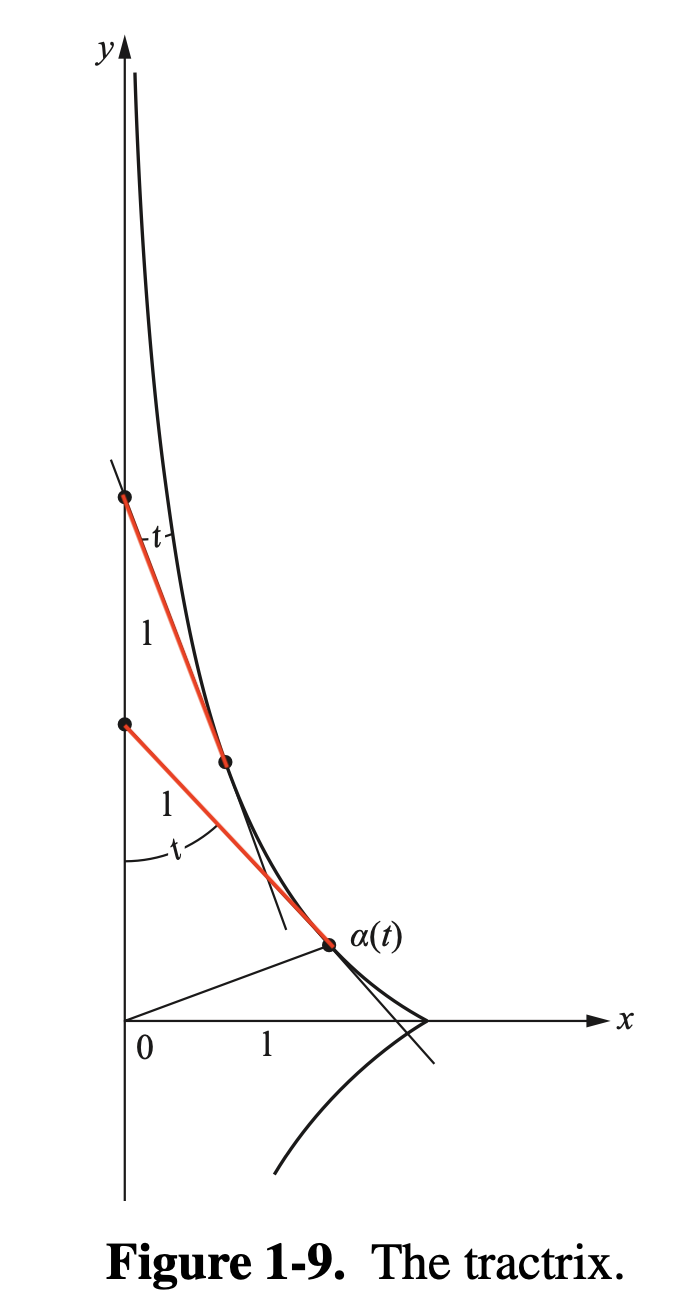
\includegraphics[scale=0.5]{Problemas/tractrix.png}
        \end{figure}

        Para esto, tendremos que general la ecuación de la tangente y posteriormente calcular la longitud del segmento de la tangente a la tractriz. Consideramos: 
        $$(y-y(t))=m(x-x(t)), \quad m= \frac{\Delta y}{\Delta x}$$

        Sea
        \begin{align*}
            m=\frac{\Delta y}{\Delta x} = \frac{dy}{dx}= \frac{\frac{dy}{dt}}{\frac{dx}{dt}}= \frac{-\sin t +\frac{1}{\sin t}}{\cos t}= -\frac{\sin t}{\cos t}+\frac{1}{\sin t\cos t}
        \end{align*}
        Entonces:
        \begin{align*}
            \left(y- \left(\cos t+ \log \tan \frac{t}{2}\right)\right) &=\left(-\frac{\sin t}{\cos t}+\frac{1}{\sin t\cos t}\right)(x-\sin t)
        \end{align*}
        Consideremos ahora, el punto ($x_1,y_1$) en donde se intersecta la tractriz y la tangente. Entonces, calculemos la distancia de este punto con el origen, como: 
        \begin{align*}
            d= \sqrt{(x_1 - 0)^2 + (y_1 - 0)^2} &= \sqrt{\sin(t)^2 + \left(y_1 - \cos(t) - \log\tan\frac{t}{2}\right)^2}
        \end{align*}

Sea $x = \sin t$ y $y = y_1$, y lo reemplazamos en la ecuación de la recta: 
\begin{align*}
    \left(y- \left(\cos t+ \log \tan \frac{t}{2}\right)\right) &=\left(-\frac{\sin t}{\cos t}+\frac{1}{\sin t\cos t}\right)(x-\sin t)\\
    \left(y_1- \left(\cos t+ \log \tan \frac{t}{2}\right)\right) &=\left(-\frac{\sin t}{\cos t}+\frac{1}{\sin t\cos t}\right)(\sin t-\sin t)\\
    y_1- \left(\cos t+ \log \tan \frac{t}{2}\right)&= 0
    \intertext{Entonces, despejamos para $y_1$, tal que:}
    y_1 &= \cos t+ \log \tan \frac{t}{2}
\end{align*}
Entonces, reemplazamos en $d$, tal que: 
\begin{align*}
    d &=\sqrt{\sin(t)^2 + \left(\cos t+ \log \tan \frac{t}{2} - \cos(t) - \log\tan\frac{t}{2}\right)^2}\\
    & =\sqrt{\sin(t)^2 + \left(\cos t+ \log \tan \frac{t}{2} - \cos(t) - \log\tan\frac{t}{2}\right)^2}\\
    & =\sqrt{\sin(t)^2 + \left(0\right)^2}\\
    &= \left|\sin t \right|\\
    &= 1
\end{align*}

    \end{sol}
\end{itemize}


\end{problema}

\begin{problema}
    
    Sea $\alpha$ una curva plana regular en coordenadas polares $(r, \varphi)$, dada por $r=r(\varphi)$. Usando la notación $r^{\prime}=\frac{\partial r}{\partial \varphi}$, verificar que la longitud de arco en el intervalo $\left[\varphi_{1}, \varphi_{2}\right]$ es

$$
s=\int_{\varphi_{1}}^{\varphi_{2}} \sqrt{r^{\prime 2}+r^{2}} d \varphi
$$

y que la curvatura está dada por

$$
\kappa(\varphi)=\frac{2 r^{\prime 2}-r r^{\prime \prime}+r^{2}}{\left(r^{\prime 2}+r^{2}\right)^{3 / 2}}
$$

\begin{sol}
    Considérese, $x=r\cos \varphi$ y $y=r\sin\varphi $. De esto, se genera el vector posición, 
    $$\alpha(\varphi)= \left(r\cos \varphi,r\sin \varphi\right)$$
    y su derivada: 
    $$\alpha'(\varphi)= \left(r'cos\varphi - r\sin \varphi,r'\sin \varphi +r\cos\varphi \right)$$
    Ahora, mostraremos $s$ y $\kappa$: 
    \begin{itemize}
        \item Para la longitud de arco $s$, sea: 
        \begin{align*}
            s &= \int_{\varphi_1}^{\varphi_2}|\alpha'(\varphi)|d\varphi\\
              &= \int_{\varphi_1}^{\varphi_2}\sqrt{(r'cos\varphi - r\sin \varphi)^2+(r'\sin \varphi +r\cos\varphi)^2}d\varphi\\
              &= \int_{\varphi_1}^{\varphi_2}\sqrt{(r'cos\varphi)+ (r\sin \varphi)^2+(r'\sin \varphi)^2 +(r\cos\varphi)^2}d\varphi\\
              &= \int_{\varphi_1}^{\varphi_2}\sqrt{r^{\prime 2}+r^{2}}d\varphi\\
        \end{align*}
        \item Para la curvatura, considérese la tercera derivada:\
        \begin{align*}
            \alpha''(\varphi) &= \left((r''\cos\varphi -r'\sin\varphi)-(r'\sin \varphi +r\cos\varphi), (r''\sin \varphi + r'\cos \varphi)+(r'\cos\varphi -r\sin\varphi )\right)\\
            &= \left(r''\cos\varphi -r'\sin\varphi-r'\sin \varphi -r\cos\varphi, r''\sin \varphi + r'\cos \varphi+r'\cos\varphi -r\sin\varphi \right)\\
            &= \left(r''\cos\varphi -r'\sin\varphi-r'\sin \varphi -r\cos\varphi, r''\sin \varphi + r'\cos \varphi+r'\cos\varphi -r\sin\varphi \right)\\
            &= \left((r''-r)\cos \varphi -2r'\sin\varphi, (r''-r)\sin\varphi +2r'\cos\varphi \right)\\
        \end{align*}
        Por medio del \textbf{Problema 8}, se tiene para una curva plana, su curvatura dada por: 
        \begin{align*}
            \kappa(t) &= \frac{\det(\alpha ', \alpha'')}{|\alpha '|^3}\\
                      &= \frac{|\alpha'\times \alpha''|}{|\alpha '|^3}\\
                      &= \frac{x'y''-y'x''}{\left(\sqrt{x'^2+y'^2}\right)^3}\\
                      &= \frac{\splitfrac{\left(r'cos\varphi - r\sin \varphi\right)\left((r''-r)\sin\varphi +2r'\cos\varphi\right)-}{-\left(r'\sin \varphi +r\cos\varphi\right)\left((r''-r)\cos \varphi -2r'\sin\varphi\right)}}{\left(\sqrt{\left(r'cos\varphi - r\sin \varphi\right)^2+\left(r'\sin \varphi +r\cos\varphi\right)^2}\right)^3}\\
                      &= \frac{\splitfrac{\left(r'cos\varphi - r\sin \varphi\right)(r''-r)\sin\varphi + \left(r'cos\varphi - r\sin \varphi\right)\left(2r'\cos\varphi\right)-}{-\left(r'\sin \varphi +r\cos\varphi\right) (r''-r)\cos \varphi +\left( 2r'\sin\varphi\right)\left(r'\sin \varphi +r\cos\varphi\right)}}{\left(\sqrt{\left(r'cos\varphi - r\sin \varphi\right)^2+\left(r'\sin \varphi +r\cos\varphi\right)^2}\right)^3}\\
                      &=\frac{2r'^2 -rr'' +r^2}{\left(r'^2 +r^2\right)^{3/2}}
        \end{align*}
        
    \end{itemize}
\end{sol}

\end{problema}


\begin{problema}
    Calcular la curvatura de la espiral de Arquímedes, la cual está dada por $r(\varphi)=a \varphi, a$ constante (Figura $1(a))$.
    \begin{sol}
        Sea
        \begin{align*}
            r'(\varphi) &= a\\
            r''(\varphi) &= 0
        \end{align*}
        Considerando el \textbf{Problema 4}, tenemos: 
        \begin{align*}
            \kappa(\varphi)&=\frac{2 r^{\prime 2}-r r^{\prime \prime}+r^{2}}{\left(r^{\prime 2}+r^{2}\right)^{3 / 2}}\\
            &= \frac{2a^2-0+(a\varphi)^2}{(a^2+(a\varphi)^2)^{3/2}}\\
            &= \frac{a^2(2+\varphi^2)}{(a^2(1+\varphi^2))^{3/2}}\\
            &= \frac{(2+\varphi^2)}{a^{3}(1+\varphi^2)^{3/2}}\\
        \end{align*}
    \end{sol}
\end{problema}

\begin{problema}
     Para la espiral logarítmica, dada en coordenadas polares por por $r(t)=a e^{t}, \varphi(t)=b t, a, b$ constantes (Figura $\left.1(b)\right)$, probar lo siguiente:
\begin{enumerate}
    \item La longitud de la curva en el intervalo $(-\infty, t]$ es proporcional al radio $r(t)$
    \begin{sol}
        Considere:
        $$r(t) = ae^t$$
        De esto, 
        \begin{align*}
            r(\varphi) &=ae^{\frac{\varphi}{b}}\\
            r'(\varphi) &= \frac{\partial (r(\varphi))}{\partial \varphi  }\\
            &= a\frac{\partial }{\partial \varphi }\left(e^{\frac{\varphi}{b}}\right)\\
            &= \frac{a}{b}\cdot\left(e^{\frac{\varphi}{b}}\right)\\
            &= \frac{ae^{\phi/b}}{b}
        \end{align*}
        La longitud de arco de la curva se define como: 
        \begin{align*}
            s &= \int_{\varphi_{1}}^{\varphi_{2}} \sqrt{r^{\prime 2}+r^{2}} d \varphi= \int_{\varphi_{1}}^{\varphi_{2}} \sqrt{\left(\frac{ae^{\phi/b}}{b}\right)^{2}+\left(ae^{\phi/b}\right)^{2}} d \varphi\\
            &= \int_{\varphi_{1}}^{\varphi_{2}} \sqrt{\left(ae^{\phi/b}\right)^{2}\left(\frac{1}{b^2}+1\right)} d \varphi= \int_{\varphi_{1}}^{\varphi_{2}} \left(ae^{\phi/b}\right)\sqrt{\left(\frac{1}{b^2}+1\right)} d \varphi\\
            &= a\sqrt{\left(\frac{1}{b^2}+1\right)}\int_{\varphi_{1}}^{\varphi_{2}} \left(e^{\phi/b}\right) d \varphi= a\sqrt{\left(\frac{1}{b^2}+1\right)} \left[be^{\varphi/b}\right]_{\varphi_1}^{\varphi_2}\\
            &=ab\sqrt{\left(\frac{1}{b^2}+1\right)} \left[e^{\varphi_2/b}-e^{\varphi_1/b}\right]\\
        \end{align*}
        Cuando $\varphi_2=t$ y $\varphi_1=-\infty$:
        \begin{align*}
            s &= ab\sqrt{\left(\frac{1}{b^2}+1\right)} \left[e^{t/b}-0\right]\\
            &= b\sqrt{\left(\frac{1}{b^2}+1\right)} \left[ae^{t/b}\right]
        \end{align*}

        Lo que demuestra que: 
        $$r(t)\propto b\sqrt{\left(\frac{1}{b^2}+1\right)} \left[ae^{t/b}\right]$$

    \end{sol}
    \item $\alpha(t) \rightarrow 0$, cuando $t \rightarrow -\infty$ y $\alpha$ tiene longitud de arco finita en el intervalo $(-\infty, t_0]$.
    \begin{cajita}
        A este problema se le hizo la corrección del infinito negativo, ya que en caso contrario $\alpha(t)$ nunca se va a 0, ni la longitud es finita. 
    \end{cajita}
    \begin{sol}
        Sea $\alpha(t)$ el vector posición. Tenemos: 
        $$r(t)= ae^{t}$$

        Para encontrar $\alpha(t)$, entonces considérese $x=r\cos t$ y $y=r\sin t$. Entonces: 
        \begin{align*}
            \alpha(t) & =(r(t)\cos t,r(t)\sin t)\\
                      &= (ae^{t}\cos t,ae^{t}\sin t)\\
        \end{align*}

        Además, 
        \begin{align*}
            \alpha'(t) &= \left(a\left(e^{t}\cos t - e^{t}\sin t \right),a\left(e^{t}\sin t+ e^{t}\cos t \right) \right)\\
            &= \left(ae^{t}\left(\cos t -\sin t \right),ae^{t}\left(\sin t+ \cos t \right) \right)\\
        \end{align*}


        Debemos demostrar: 
        \begin{enumerate}
            \item $\lim_{t\to -\infty} a(t)=0$. Nótese: 
            \begin{align*}
                \lim_{t\to -\infty} a(t) &= \lim_{t\to -\infty} (ae^{t}\cos \theta,ae^{t}\sin \theta)\\
                &= (0,0)=0
            \end{align*}
            \item $\alpha(t)$ tiene longitud de arco finita en el intervalo $(-\infty, t_0]$: 
            \begin{align*}
                s &= \int_{-\infty}^{t_0} \sqrt{\left(x'(t)\right)^2+\left(y'(t)\right)^2}dt\\
                &= \int_{-\infty}^{t_0} \sqrt{\left(ae^{t}\left(\cos t -\sin t \right)\right)^2+\left(ae^{t}\left(\sin t+ \cos t \right)\right)^2}dt\\
                &= \int_{-\infty}^{t_0} ae^{t}\sqrt{\left(\cos t -\sin t \right)^2+\left(\sin t+ \cos t \right)^2}dt\\
                &= \int_{-\infty}^{t_0} ae^{t}\sqrt{2\left(cos^2t +\sin^2t\right)}dt\\
                &= \int_{-\infty}^{t_0} ae^{t}\sqrt{2}dt\\
                & = a\sqrt{2} \left[e^t\right]_{-\infty}^{t_0} = a\sqrt{2} e^{t_0}\\
            \end{align*}
            Mostrando que en efecto la longitud de arco es finita.
        \end{enumerate}
        
    \end{sol}
    \item El vector $\alpha(t)$ tiene ángulo constante con el vector tangente $\alpha^{\prime}(t)$.
    \begin{sol}
        Nótese, 
        \begin{align*}
            \alpha(t) &= (ae^{t}\cos t,ae^{t}\sin t)\\
            \alpha'(t) &= \left(ae^{t}\left(\cos t -\sin t \right),ae^{t}\left(\sin t+ \cos t \right) \right)
        \end{align*}
        Ahora, considérese la propiead: 
        $$A\cdot B = |A||B|\cos\theta_{AB}\implies \theta_{AB}=\arccos\left(\frac{A\cdot B}{|A||B|}\right)$$
        Entonces, 
        \begin{align*}
            \theta_{AB}&=\arccos\left(\frac{A\cdot B}{|A||B|}\right)\\
            &= \arccos\left(\frac{(ae^{t})^2(\cos^2t -\cos t \sin t)+(ae^{t})^2(\sin^2 t +\cos t \sin t )}{\sqrt{(ae^{t}\cos t)^2+(ae^{t}\sin t)^2}\sqrt{(ae^{t}\left(\cos t -\sin t \right))^2+(ae^{t}\left(\sin t+ \cos t \right))^2}}\right)\\
            &= \arccos\left(\frac{(ae^t)^2}{ae^t\sqrt{(ae^t)^2 (2(\cos^2 t+\sin^2 t))}}\right)\\
            &= \arccos\left(\frac{1}{\sqrt{2}}\right)\\
            &= \frac{\pi}{4}
        \end{align*}
    \end{sol}
    
\end{enumerate}

\end{problema}

\begin{figure}[H]
    \centering
    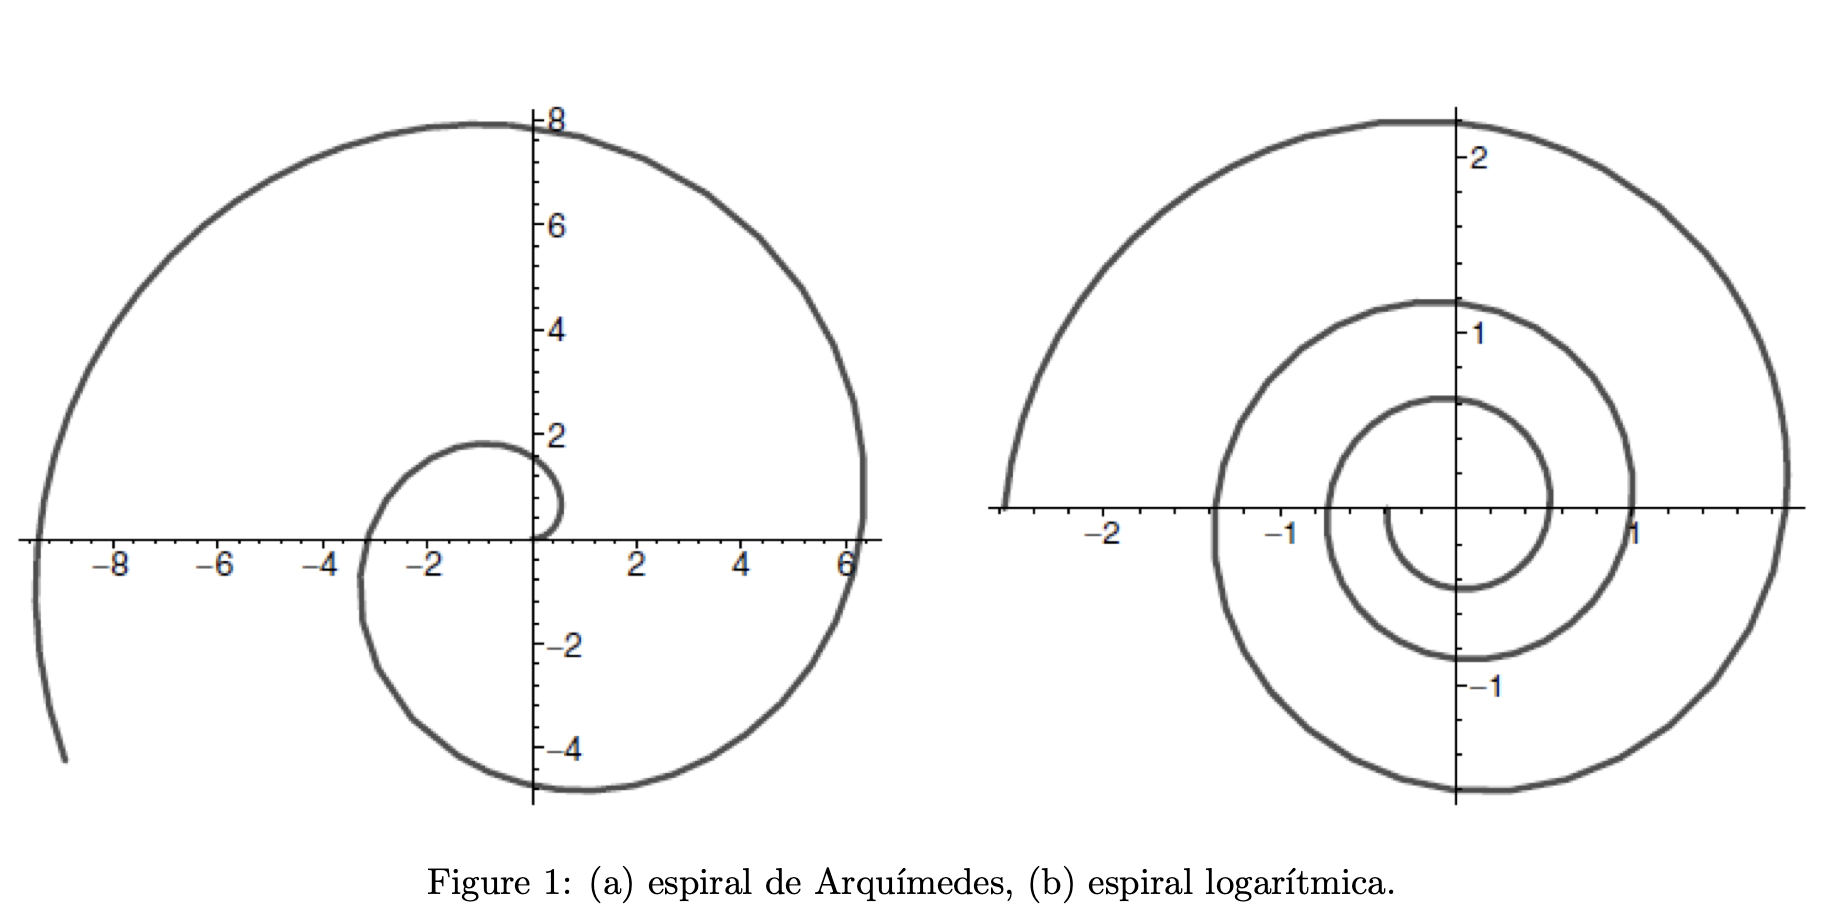
\includegraphics[scale=0.5]{Problemas/gf.png}
\end{figure}


\begin{problema}
    Mostrar que la curva de menor longitud entre dos puntos $\mathbf{p}, \mathbf{q} \in \mathbb{R}^{n}$ es el segmento de recta que los une. (Sugerencia: ver las ideas en el Ejercicio 10, pág 11 de Do Carmo.) 
    \begin{sol}
        Sea $\alpha: I\to \mathbb{R}^n$ una curva parametrizada. Sea $[a,b]\subset I$ y sea $\alpha(a)=p$ y $\alpha(b)=q$, tal que debemos probar: 
        $$|\alpha(b)-\alpha(a)|\leq \int_a^b |\alpha'(t)|dt$$
        \begin{itemize}
            \item Primero, debemos mostrar la siguiente propiedad: para cualquier vector constante $v$, $|v|=1$, 
            $$(q-p)\cdot v= \int_{a}^{b}\alpha'(t)\cdot vdt \leq \int_{a}^{b}|\alpha '(t)|dt$$
            \begin{itemize}
                \item Sea
                    \begin{align*}
                        \int_{a}^{b}\alpha'(t)\cdot vdt &= \int_{a}^{b}\left(\alpha_1'(t)v_1+\alpha_2'(t)v_2+\cdots +\alpha_n'(t)v_n\right) dt\\
                        &= \left[\alpha_1(t)v_1+\alpha_2(t)v_2+\cdots +\alpha_n(t)v_n\right]_{a}^b\\
                        &= \left[\alpha_1(b)v_1+\alpha_2(b)v_2+\cdots +\alpha_n(b)v_n\right]-\\
                        & \ \ \ \ -\left[\alpha_1(a)v_1+\alpha_2(a)v_2+\cdots +\alpha_n(a)v_n\right]\\
                        &= \alpha(b)\cdot v - \alpha(a)\cdot v\\
                        &= v\cdot (\alpha(b) - \alpha(a))\\
                        &= v\cdot (p-q)\\
                        &= (p-q)\cdot v
                    \end{align*}
                \item Sea 
                    \begin{align*}
                        \int_{a}^{b}\alpha'(t)\cdot vdt &\leq \left|\int_{a}^{b}\alpha'(t)\cdot vdt\right|\\
                        &\leq \int_{a}^{b}|\alpha'(t)\cdot v|dt\\
                        &\leq \int_{a}^{b}|\alpha'(t)|\cdot \underbrace{|v|}_{1}dt\\
                        &= \int_{a}^{b}|\alpha'(t)|dt
                    \end{align*}
            \end{itemize}
            \item Segundo, procedemos a la curva de menor longitud entre dos puntos $p,q$. Sea, 
                \begin{align*}
                    |\alpha(b)-\alpha(a)| &= |q-p|\\
                                          &= \frac{|q-p|^2}{|q-p|}\\
                                          &= \frac{(q-p)\cdot (q-p)}{|q-p|}\\
                                          &= (q-p)\cdot v
                    \intertext{Y por la parte uno: }
                    &\leq  \int_{a}^{b}|\alpha'(t)|dt
                \end{align*}
        \end{itemize}


   \end{sol}
    
\end{problema}

\begin{problema}
Probar que la curvatura y la torsión de una curva de Frenet $\alpha(t)$ en $\mathbb{R}^{3}$, parametrizada de forma arbitraria, están dadas por

$$
\kappa(t)=\frac{\left|\alpha^{\prime} \times \alpha^{\prime \prime}\right|}{\left|\alpha^{\prime}\right|^{3}}, \quad \tau(t)=\frac{\operatorname{det}\left(\alpha^{\prime}, \alpha^{\prime \prime}, \alpha^{\prime \prime \prime}\right)}{\left|\alpha^{\prime} \times \alpha^{\prime \prime}\right|^{2}} .
$$

En particular, en el caso de curvas planas,

$$
\kappa(t)=\frac{\operatorname{det}\left(\alpha^{\prime}, \alpha^{\prime \prime}\right)}{\left|\alpha^{\prime}\right|^{3}} .
$$

(Sugerencia: ver las ideas en el Ejercicio 12, pág 26 de Do Carmo.)
\begin{sol}
    
\end{sol}
\end{problema}

\begin{problema}Sea $\alpha$ la hélice en $\mathbb{R}^{3}$, dada por

$$
\alpha(t)=(a \cos t, a \sin t, b t), \quad a, b \in \mathbb{R}^{+} .
$$

Muestre que la curvatura y la torsión de $\alpha$ son constantes.
\begin{sol}
    Sea 
    \begin{align*}
        \alpha'(t) &= \frac{d}{dt}(a \cos t, a \sin t, b t)\\
                   &= (-a \sin t, a \cos t, b)
        \intertext{también,}
        \alpha''(t) &= \frac{d}{dt}(-a \sin t, a \cos t, b)\\
                   &= (-a \cos t, -a \sin t, 0)
        \intertext{Además,}
        \alpha'''(t) &= \frac{d}{dt}(-a \cos t, -a \sin t, 0)\\
                   &= (a \sin t, -a \cos t, 0)
    \end{align*}
    Ahora bien,
    \begin{itemize}
        \item La curvatura: 
        \begin{align*}
            \kappa(t)&=\frac{\left|\alpha^{\prime} \times \alpha^{\prime \prime}\right|}{\left|\alpha^{\prime}\right|^{3}}\\
            &= \frac{\left|\begin{bmatrix}
                -a \sin t & a \cos t & b\\
                -a \cos t & -a \sin t & 0
            \end{bmatrix}\right|}{\left(\sqrt{(-a\sin t)^2+(a\cos t)^2+b^2}\right)^3}\\
            &= \frac{\left|\left(0+ab\sin t,-(0+ab\cos t),a^2\sin^2t+a^2\cos^2t\right)\right|}{\left(\sqrt{a^2+b^2}\right)^3}\\
            &= \frac{1}{\left(\sqrt{a^2+b^2}\right)^3}\left|\left(ab\sin t, -ab\cos t, a^2\right)\right|\\
            &= \frac{1}{\left(\sqrt{a^2+b^2}\right)^3}\sqrt{(ab\sin t)^2+ (-ab\cos t)^2+( a^2)^2}\\
            &= \frac{1}{\left(\sqrt{a^2+b^2}\right)^3}\sqrt{a^2(b^2+a^2)}\\
        \end{align*}
        \item La torsión: 
        \begin{align*}
            \tau(t)&=\frac{\operatorname{det}\left(\alpha^{\prime}, \alpha^{\prime \prime}, \alpha^{\prime \prime \prime}\right)}{\left|\alpha^{\prime} \times \alpha^{\prime \prime}\right|^{2}}\\
            &=\frac{(\alpha' \times  \alpha'')\cdot \alpha'''}{\left|\alpha^{\prime} \times \alpha^{\prime \prime}\right|^{2}}\\
            &= \frac{\left(ab\sin t, -ab\cos t, a^2\right)\cdot(a \sin t, -a \cos t, 0) }{|\left(ab\sin t, -ab\cos t, a^2\right)|^2}\\
            &= \frac{1}{a^2(b^2+a^2)}(a^2b\sin^2t +a^2b\cos^2t )\\
            &= \frac{a^2b}{a^2(b^2+a^2)}\\
            &= \frac{b}{(b^2+a^2)}\\
        \end{align*}
    \end{itemize}
\end{sol}
\end{problema}

\begin{problema}
     Construir una curva plana, parametrizada por longitud de arco, cuya curvatura esté dada exactamente por $\kappa(s)=s^{-1 / 2}=1/s^{1/2}=1/\sqrt{s}$.
    \begin{sol}
        Usando el procedimiento del \textbf{Teorema Fundamental de las Curvas Planas}, tenemos que la curva se puede construir a partir de la expresión 
        $$\alpha(s)=\left(\int_{s_0}^{s}\cos(\theta(u))du,\int_{s_0}^{s}\sin(\theta(u))du\right), \quad s_0\in I$$
        en donde $\theta: I\to\mathbb{R}$ tal que $\theta(u)=\int_{s_0}^{u}\kappa_0(t)dt$. Primero, definimos $s_0=0$, y hacemos un cambio de variable tal que $k(t)=1/\sqrt{t}$. Entonces, 
        \begin{align*}
            \theta(u)&=\int_{0}^{u}\frac{1}{\sqrt{t}}dt\\
            &= 2\sqrt{u}
        \end{align*}
        De esto: 
        \begin{align*}
            \alpha(s)&=\left(\int_{0}^{s}\cos(2\sqrt{u})du,\int_{0}^{s}\sin(2\sqrt{u})du\right)\\
            &= \left(\sqrt{u}\sin(2\sqrt{u})+\frac{1}{2}\cos (2\sqrt{u})\Big|_0^s,\frac{1}{2}\sin(2\sqrt{u})-\sqrt{u}\cos(2\sqrt{u})\Big|_0^s\right)\\
            &= \left(\sqrt{s}\sin(2\sqrt{s})+\frac{1}{2}\cos (2\sqrt{s})-\frac{1}{2},\frac{1}{2}\sin(2\sqrt{s})-\sqrt{s}\cos(2\sqrt{s})\right)\\
        \end{align*}


       
    \end{sol}
\end{problema}

%---------------------------
%\bibliographystyle{apa}
%\bibliography{referencias.bib}

\end{document}